\chapter{Metodologi Penelitian}

\section{Deskripsi Umum Penelitian}

Studi literatur dilakukan dengan mempelajari penelitian sebelumnya yang terkait yang diperoleh dari berbagai macam sumber seperti buku, artikel, publikasi jurnal, paper, tesis, disertasi dll.

\begin{figure}[h]
    \centering
    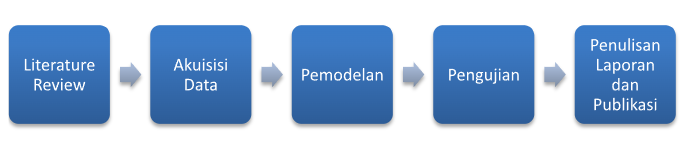
\includegraphics[width=0.8\textwidth]{contents/chapter-3/tahapan-penelitian.png}
    \caption{Contoh tahapan penelitian}
    \label{fig:tahapan-penelitian}
\end{figure}

\textcolor{red}{Catatan: Ganti gambar di atas dengan diagram tahapan penelitian Anda. Simpan file gambar di folder contents/chapter-3/ dengan nama tahapan-penelitian.png (atau format lain seperti .jpg, .pdf).}

\section{Akuisisi Data}

Sub bab ini menjelaskan tentang karakteristik data yang digunakan dalam penelitian. Penjelasan dapat dimulai dengan bagaimana data diperoleh jika menggunakan data primer yang diambil secara langsung, atau dari mana sumber data diperoleh jika menggunakan data sekunder yang tersedia secara publik. 

Kemudian, karakteristik data perlu dijelaskan dengan menyebutkan jumlah data yang digunakan, seperti apa isi dari data beserta representasinya, dan visualisasi contoh dari data. 

Terakhir, perlu dijelaskan bagaimana data dibagi ke dalam beberapa subdata seperti data pelatihan, data validasi, dan data uji dalam bentuk tabel. Jika ada proses data augmentasi (data tambahan berdasar data yang ada) maka metode yang digunakan juga perlu dijelaskan.

\section{Rancangan Metode/Model/Algoritma}

Bagian ini berisi penjelasan detail tentang metode/model/desain yang digunakan dalam penelitian. Pembahasan diawali dengan penjelasan secara umum tahap-tahap metode/model/desain/algoritma yang dilengkapi dengan bagan alir, kemudian setiap sub-bab menjelaskan lebih detail setiap tahapan yang disertai dengan sumber referensi yang terkait, ilustrasi/bagan/bagan alir bagaimana tahap dilakukan, dan persamaan-persamaan yang digunakan. 

Dalam rancangan metode ini yang dideskripsikan bisa berupa algoritma, perangkat lunak, perangkat keras atau hal lainnya yang terkait dengan penelitian. Berikut adalah salah satu contoh kerangka penulisan untuk kasus Estimasi Umur Berbasis Citra Wajah Menggunakan Ciri Tekstur dan Metode Support Vector Machine:

\subsection{Overview Metode/Model/Algoritma}

\begin{figure}[h]
    \centering
    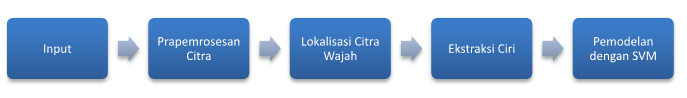
\includegraphics[width=0.8\textwidth]{contents/chapter-3/overview-metode.png}
    \caption{Contoh overview metode}
    \label{fig:overview-metode}
\end{figure}

\textcolor{red}{Catatan: Ganti gambar di atas dengan diagram overview metode Anda. Simpan file gambar di folder contents/chapter-3/ dengan nama overview-metode.png.}

\subsection{Prapemrosesan Citra}

Jelaskan tahapan prapemrosesan yang dilakukan pada data citra, seperti normalisasi, resizing, filtering, dll. Sertakan persamaan matematika jika diperlukan.

\subsection{Lokalisasi Citra Wajah}

Jelaskan metode yang digunakan untuk mendeteksi dan melokalisasi wajah pada citra. Sertakan referensi metode yang digunakan.

\subsection{Ekstraksi Ciri Tekstur}

Jelaskan metode ekstraksi fitur yang digunakan, seperti LBP, HOG, SIFT, dll. Sertakan persamaan dan ilustrasi jika diperlukan.

\subsection{Model Support Vector Machine}

Jelaskan arsitektur model yang digunakan, parameter-parameter yang diatur, dan proses pelatihan model.

\textcolor{red}{Catatan: Sesuaikan sub-sub bab di atas dengan metode/algoritma yang Anda gunakan dalam penelitian. Hapus atau tambahkan sub bab sesuai kebutuhan.}

\section{Rancangan Pengujian dan Evaluasi}

Bagian ini berisi penjelasan tentang bagaimana pengujian dan analisis pada metode/model yang diusulkan dalam penelitian dilakukan. Pada bagian pengujian, penjelasan bisa berupa tahap/langkah/skenario pengujian, validasi dan alat yang digunakan, sedangkan pada bagian analisis menjelaskan protokol/evaluation metrics. 

Rancangan pengujian dan analisis perlu disertai dengan sumber referensi terkait. Analisis yang dilakukan harus berupa analisis kuantitatif (akurasi, performa, waktu pemrosesan, kompleksitas, dll) dan dapat juga disertai dengan analisis kualitatif. Berikut adalah salah satu contoh dari kerangka rancangan pengujian dan analisis pada kasus pencarian objek pada video menggunakan Oriented Fast and Rotated Brief:

\subsection{Protokol Evaluasi/Metrik}

Jelaskan metrik evaluasi yang digunakan seperti akurasi, presisi, recall, F1-score, RMSE, MAE, dll. Sertakan persamaan untuk setiap metrik.

Contoh:
\begin{equation}
    \text{Akurasi} = \frac{\text{Jumlah Prediksi Benar}}{\text{Total Jumlah Data}} \times 100\%
\end{equation}

\subsection{Rancangan Pengujian terhadap Variasi Jumlah Fitur}

Jelaskan skenario pengujian dengan memvariasikan jumlah fitur yang digunakan. Buat tabel yang menunjukkan variasi parameter yang akan diuji.

\subsection{Rancangan Pengujian terhadap Variasi Jumlah Poin Utama}

Jelaskan skenario pengujian dengan memvariasikan jumlah poin utama (keypoints) yang digunakan.

\subsection{Rancangan Pengujian terhadap Ketepatan Waktu}

Jelaskan bagaimana pengujian waktu komputasi dilakukan, termasuk spesifikasi perangkat keras yang digunakan.

\textcolor{red}{Catatan: Sesuaikan sub-sub bab pengujian di atas dengan skenario pengujian yang relevan dengan penelitian Anda. Hapus atau tambahkan sub bab sesuai kebutuhan.}
